\documentclass[10pt, twocolumn]{article}
\usepackage{graphicx}
\usepackage{amsmath,amsthm}

\graphicspath{{/home/tmiles/Code/Numerical_Programming/A2/report/gfx/}}

\begin{document}
\begin{titlepage}
   \begin{center}
       \vspace*{1cm}
 
       \textbf{Numerical Programming Assignment 2}
 
       \vspace{0.5cm}
        Thomas Miles
 
       \vspace{1.5cm}
 
       \textbf{626263}
 
       \vfill
 

       \vspace{0.8cm}

 
   \end{center}
\end{titlepage}

\setcounter{section}{1}
\section{Root finding}
	\setcounter{subsection}{1}
	\subsection{Graphical Solution}
	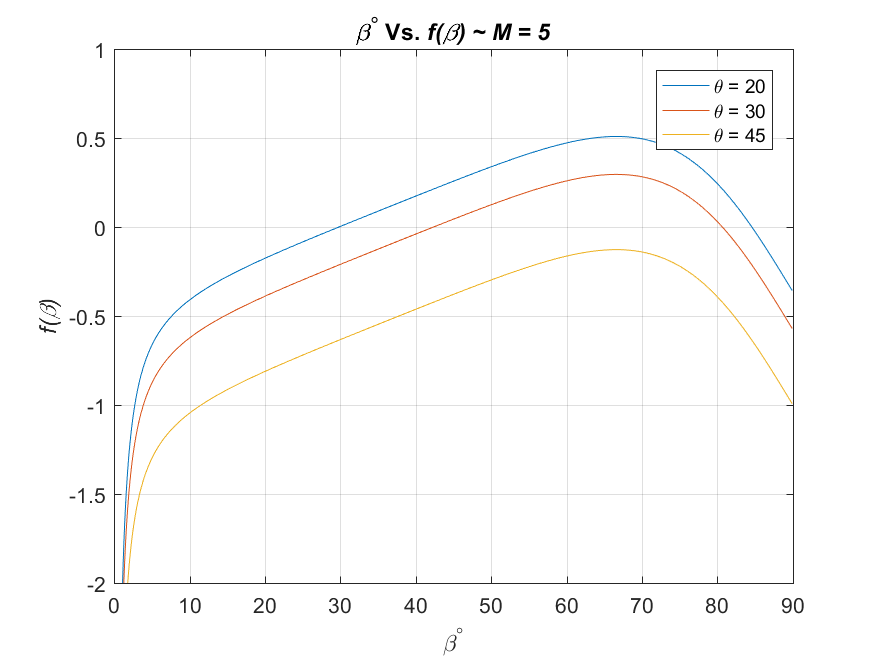
\includegraphics[scale=0.3]{5}
	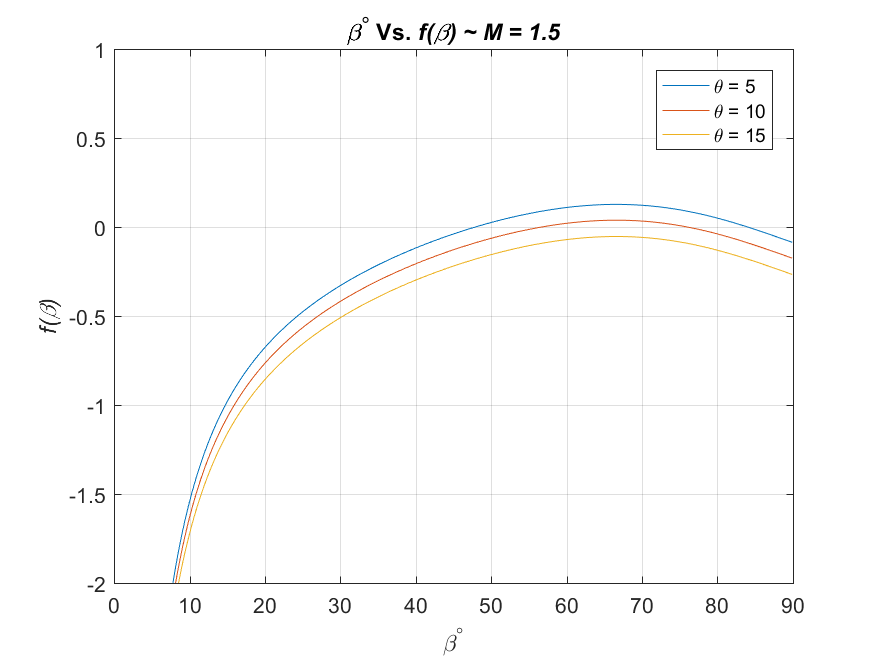
\includegraphics[scale=0.3]{15}

	The figures above demonstrate how \textit{f}($\beta$) varies when $\theta$ and M change. It can be seen that increasing $\theta$ causes a downward translation of the function. $\theta_{max}$ is the largest $theta$ for which \textit{f}($beta$) has a solution. The graphs show that for M = 5, \textit{f}($beta$) never crosses the axis at $\theta = 45^{\circ}$, so $\theta_{max} \approx 40^{\circ}$. Reducing M to 1.5 is shown to lower $\theta_{max}$, which can be estimated to be $\approx 12^{\circ}$. 
	
	\subsection{Solving the shock-wave equation}
		\subsubsection*{\quad(b)}
		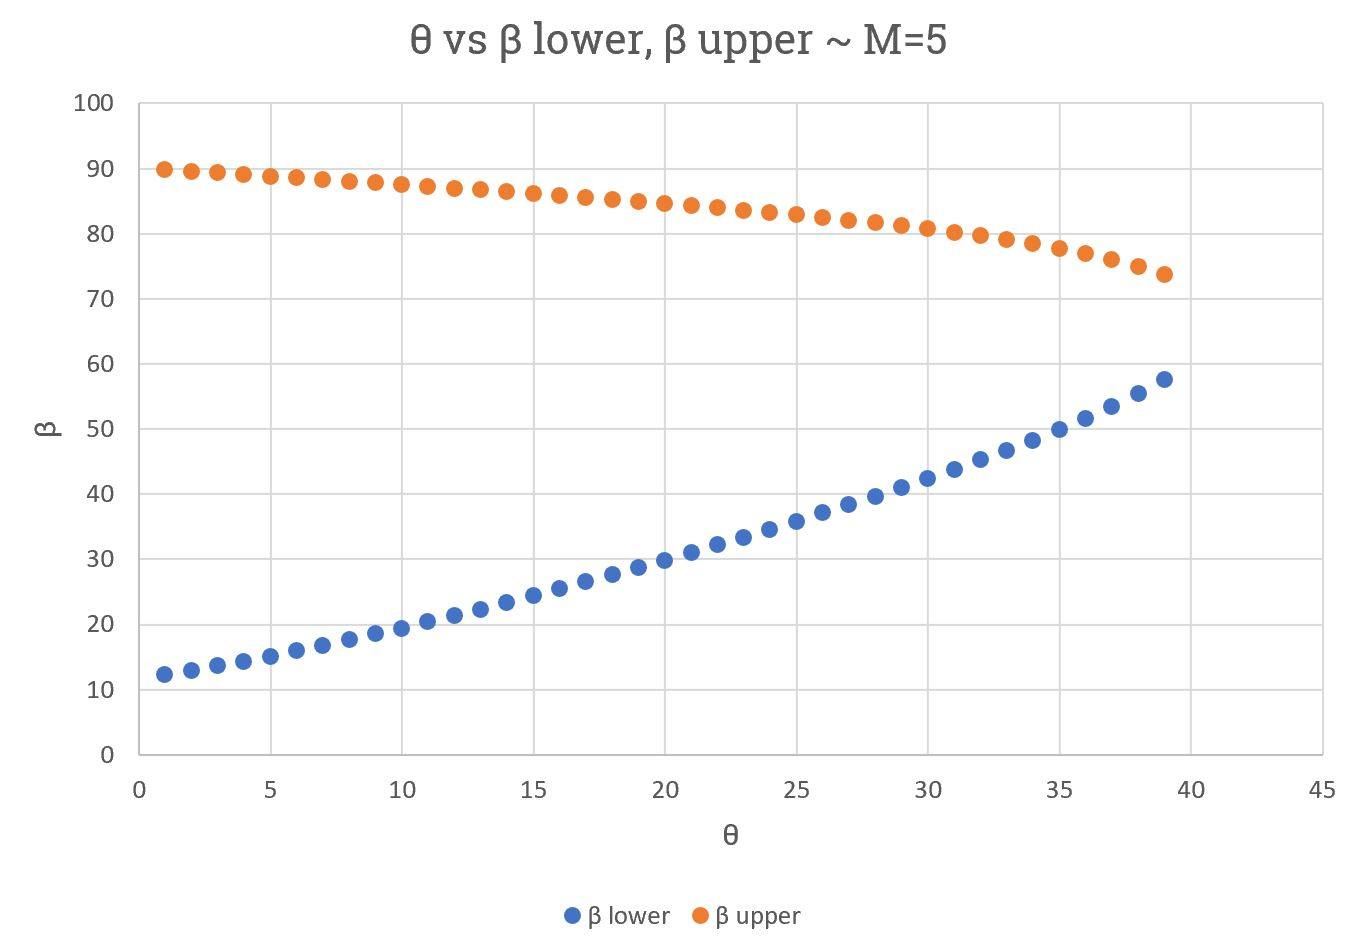
\includegraphics[scale=0.19]{bt}
		\subsubsection*{\quad(c)}
		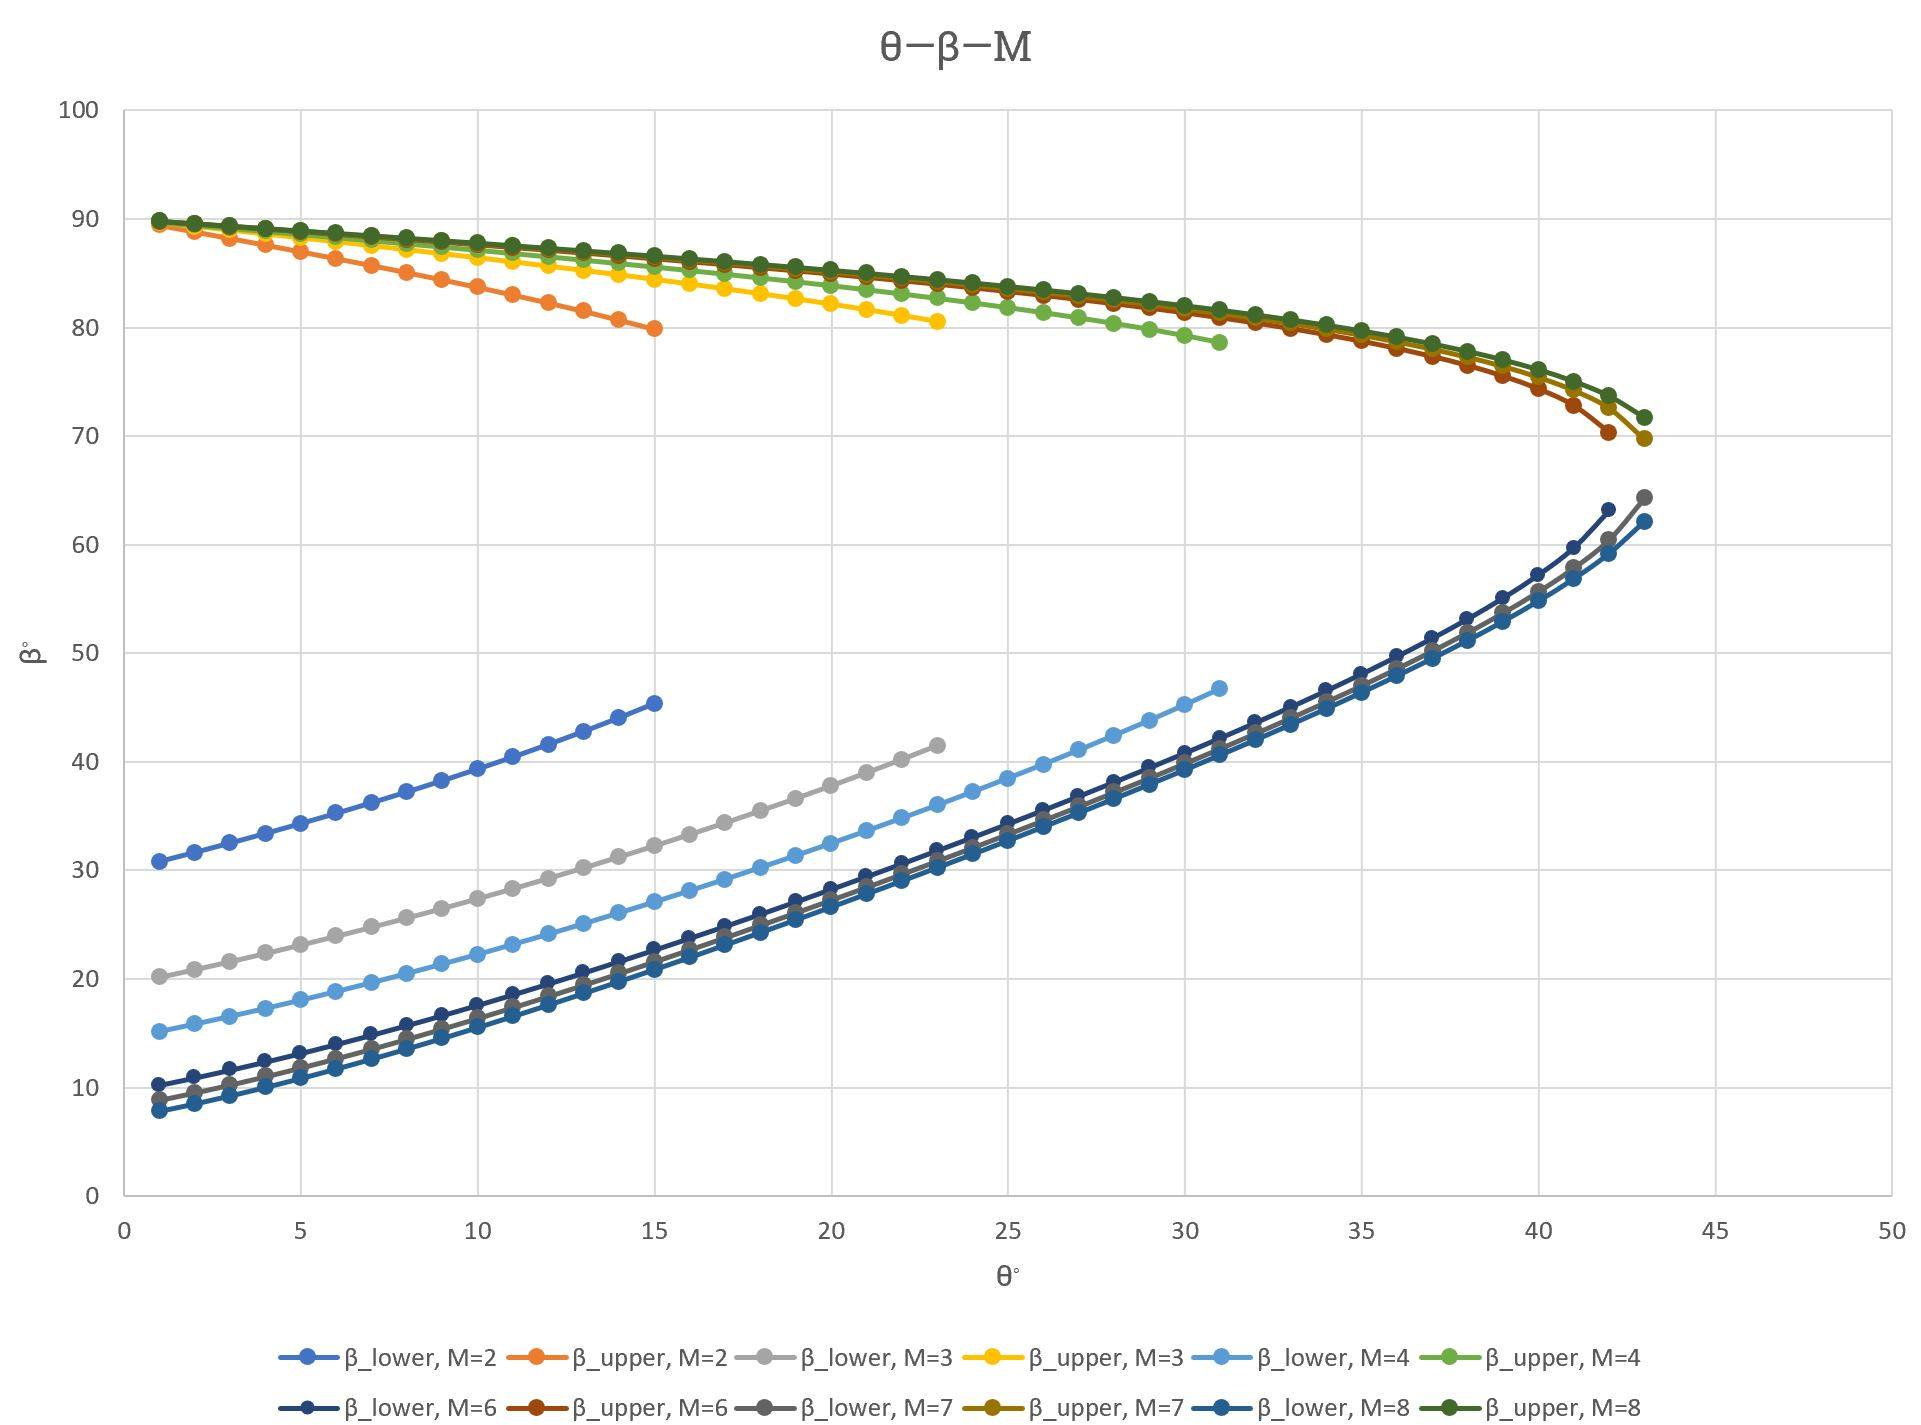
\includegraphics[scale=0.15]{tbm}

	\subsection{Solving the shock-wave equation}


\section{Regression}
Given that:
\begin{align*}
	\begin{bmatrix}
		\sum_{i=1}^{N}x_i^2 	& 	\sum_{i=1}^{N}x_i\\\\
		\sum_{i=1}^{N}x_i 		&	N
	\end{bmatrix}
	\begin{bmatrix}
	a\\\\
	b
	\end{bmatrix}
	&= 
	\begin{bmatrix}
		\sum_{i=1}^{N}x_iy_i\\\\
		\sum_{i=1}^{N}y_i
	\end{bmatrix}\\
	\text{let: }
	\begin{bmatrix}
		\sum_{i=1}^{N}x_i^2 	& 	\sum_{i=1}^{N}x_i\\\\
		\sum_{i=1}^{N}x_i 		&	N
	\end{bmatrix}
	&= X\\
\end{align*}
\begin{align*}
	\Rightarrow 
	X^{-1} &= \frac{1}{N\sum_{i=1}^{N}x_i^2 - N^2\overline{x}^2}
	\begin{bmatrix}
		N					&	\sum_{i=1}^{N}x_i\\\\
		-\sum_{i=1}^{N}x_i	&	\sum_{i=1}^{N}x^2
	\end{bmatrix}\\\\
	\Rightarrow
	\begin{bmatrix}
	a\\\\
	b
	\end{bmatrix}
	&= 	\frac{1}{N\sum_{i=1}^{N}x_i^2 - N^2\overline{x}^2}
	\begin{bmatrix}
		N					&	\sum_{i=1}^{N}x_i\\\\
		-\sum_{i=1}^{N}x_i	&	\sum_{i=1}^{N}x^2
	\end{bmatrix}
	\begin{bmatrix}
		\sum_{i=1}^{N}x_iy_i\\\\
		\sum_{i=1}^{N}y_i
	\end{bmatrix} &&(1)\\\\\\
	\Rightarrow
	\begin{bmatrix}
	a\\\\
	b
	\end{bmatrix}
	&= \frac{1}{N\sum_{i=1}^{N}x_i^2 - N^2\overline{x}^2}
	\begin{bmatrix}
		N\sum_{i=1}^{N}x_iy_i	-	N^2\overline{x} \cdot\overline{y}\\\\
		-N\overline{x}\sum_{i=1}^{N}x_iy_i	-	N\overline{y}\sum_{i=1}^{N}x^2
	\end{bmatrix}\\
\end{align*}
Thus,
\begin{align*}
	a &= \frac	{N\sum_{i=1}^{N}x_iy_i	-	N^2\overline{x} \cdot\overline{y}}
				{N\sum_{i=1}^{N}x_i^2 - N^2\overline{x}^2}\\
	\Rightarrow a &= \frac	{\sum_{i=1}^{N}x_iy_i	-	N\overline{x} \cdot\overline{y}} 
						  	{\sum_{i=1}^{N}x_i^2 - N\overline{x}^2}	&&(2)\\
	\Rightarrow a &= \frac{\sum_{i=1}^{N}x_iy_i  - N\overline{x} \cdot\overline{y} - N\overline{x} \cdot\overline{y} + N\overline{x} \cdot\overline{y}} 
	{\sum_{i=1}^{N}x_i^2 - 2N\overline{x}^2 + N\overline{x}^2}\\
	\Rightarrow a &= \frac	{\sum_{i=1}^{N}x_iy_i - \overline{x}\sum_{i=1}^{N}y_i - \overline{y}\sum_{i=1}^{N}x_i + \overline{x}\cdot\overline{y}\sum_{i=1}^{N}1}
							{\sum_{i=1}^{N}x_i^2 - 2\overline{x}\sum_{i=1}^{N}x_i + \overline{x}^2\sum_{i=1}^{N}1}\\
	\Rightarrow a &= \frac	{\sum_{i=1}^{N}(x_iy_i - \overline{x}y_i - x_i\overline{y} + \overline{x}\cdot\overline{y})}
							{\sum_{i=1}^{N}(x_i^2 - 2\overline{x}x_i + \overline{x}^2)}\\
	\Rightarrow a &= \frac	{\sum_{i=1}^{N}(x_i - \overline{x})(y_i - \overline{y})}
							{\sum_{i=1}^{N}(x_i - \overline{x})^2}\\
							&\qed\\	
\end{align*}
Expanding (1) gives:
\begin{align*}
	\begin{bmatrix}
		a(\sum_{i=1}^{N}x_i^2) + b(\sum_{i=1}^{N}x_i)\\
		a(\sum_{i=1}^{N}x_i) + Nb
	\end{bmatrix}
	&=
	\begin{bmatrix}
		\sum_{i=1}^{N}x_iy_i\\\\
		\sum_{i=1}^{N}y_i
	\end{bmatrix}\\
	\Rightarrow 
	a\sum_{i=1}^{N}x_i + Nb &= \sum_{i=1}^{N}y_i\\
	\Rightarrow a\overline{x} + b &= a\overline{y}\\
	\Rightarrow b &= \overline{y} - a\overline{x}\\
	&\qed\\
\end{align*}
\pagebreak
\setcounter{section}{4}
\section{Interpolation}
	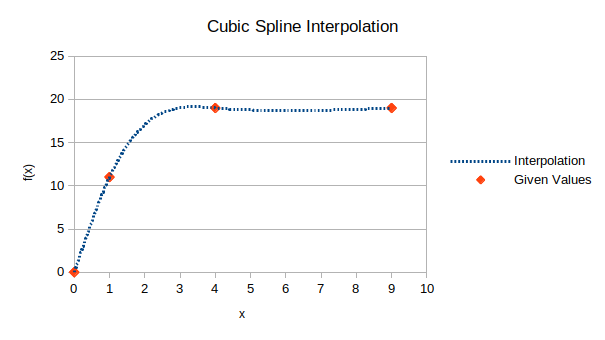
\includegraphics[scale=0.6]{spline}
	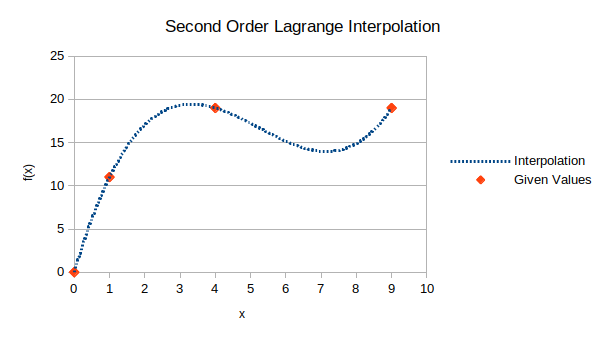
\includegraphics[scale=0.6]{lagrange}
	
	It can be seen from the plots above that the cubic spline interpolation provides a more accurate interpolation between any two data points. since each spline remains closer to each value either side of the point being estimated. With that said, if the true function representing the data points is known to be polynomial, and the data is sparse, it is possible that the Lagrange interpolation may be more accurate in certain specific cases. Furthermore, using a higher degree Lagrange interpolation would allow for fitting more closely to that of the spline method.
	
\section{Differential Equations}
\subsection*{Exact Solution}
	\includegraphics[scale=0.5]{init}
\subsection*{Euler}
	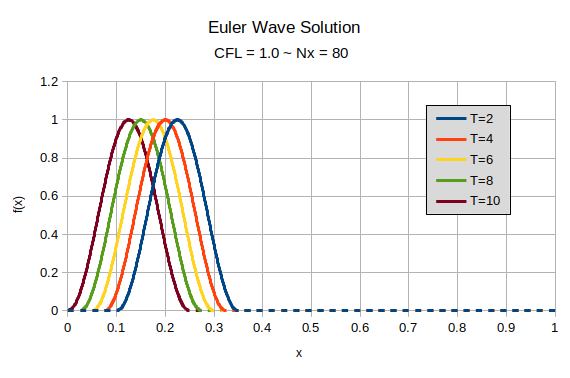
\includegraphics[scale=0.5]{eu-1-80}
	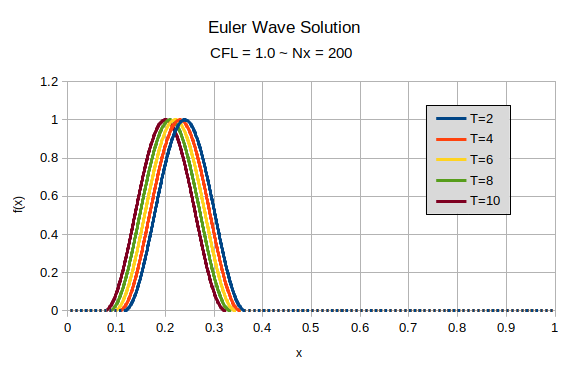
\includegraphics[scale=0.5]{eu-1-200}
	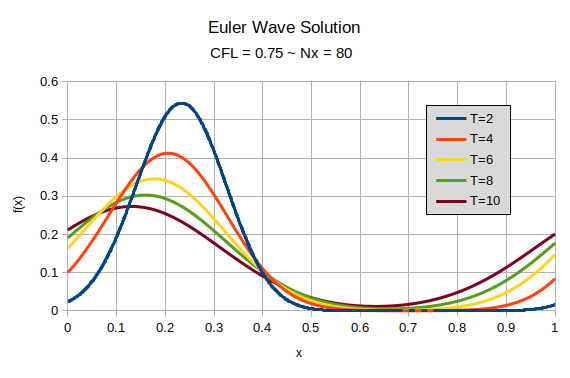
\includegraphics[scale=0.5]{eu-075-80}
	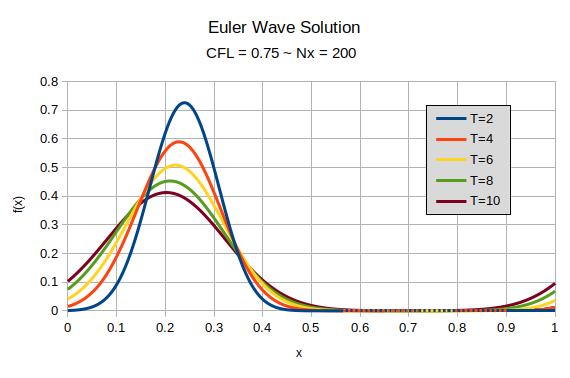
\includegraphics[scale=0.5]{eu-075-200}
	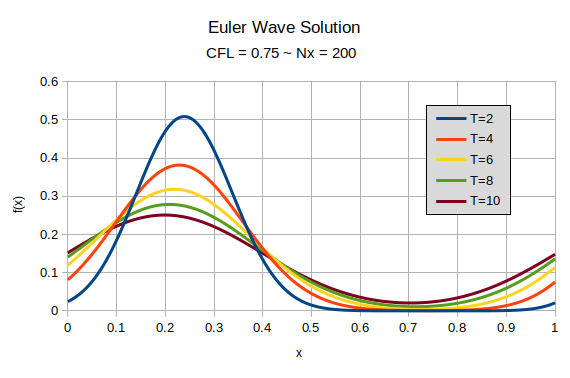
\includegraphics[scale=0.5]{eu-025-200}
	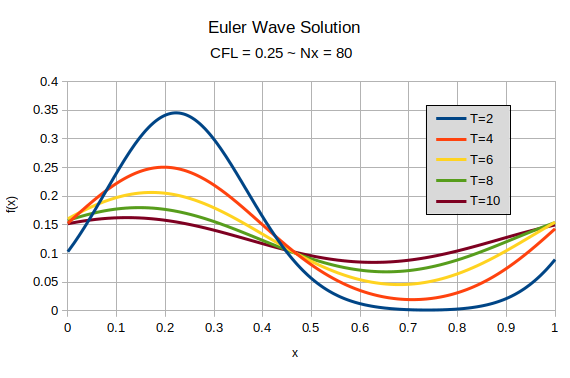
\includegraphics[scale=0.5]{eu-025-80}
	
\subsection*{Lax-Wendroff}
	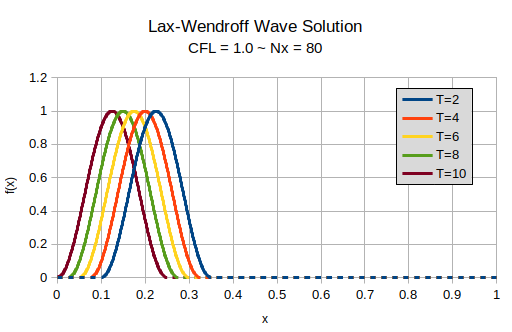
\includegraphics[scale=0.5]{lx-1-80}
	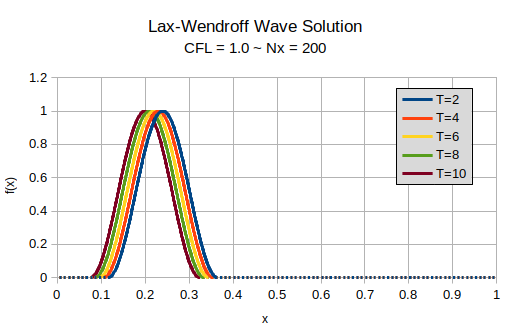
\includegraphics[scale=0.5]{lx-1-200}
	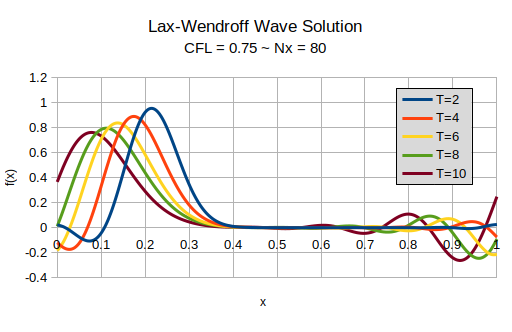
\includegraphics[scale=0.5]{lx-075-80}
	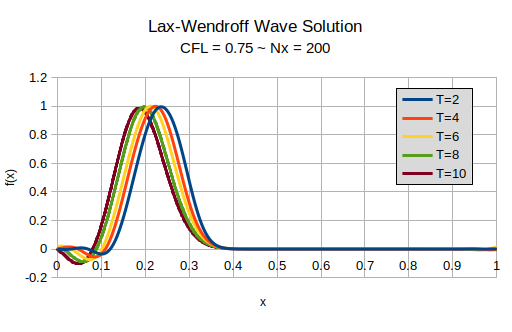
\includegraphics[scale=0.5]{lx-075-200}
	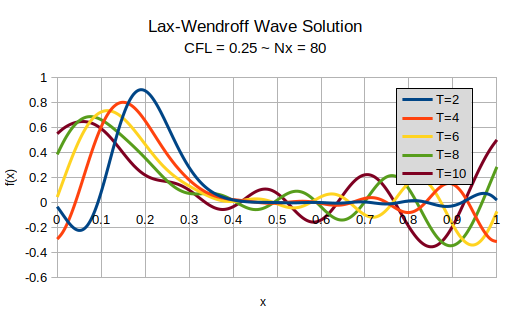
\includegraphics[scale=0.5]{lx-025-80}
	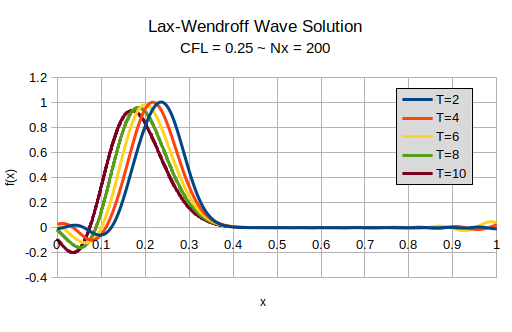
\includegraphics[scale=0.5]{lx-025-200}

\subsection*{CFL $>$ 1}
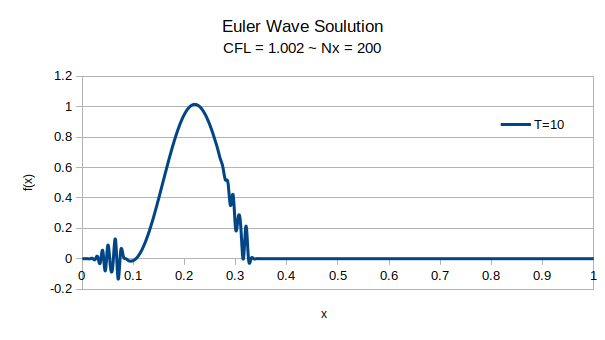
\includegraphics[scale=0.5]{eu-1002}
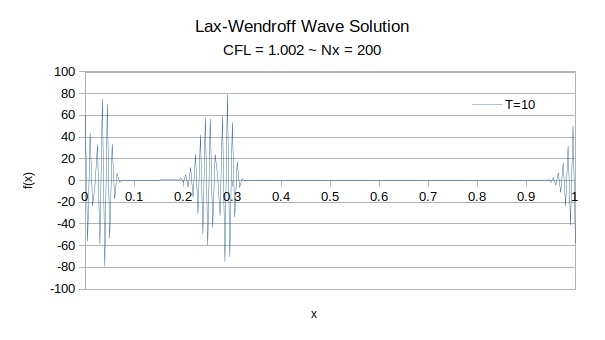
\includegraphics[scale=0.5]{lx-1002}

\subsection*{Analysis at t=10}

When comparing the graphs for both Euler and Lax-Wendroff methods, increasing $\Delta x$ results in the t=10 solution being closer to the exact solution compared to a lower precision.

For $CFL < 1$, each solution deviates further from the exact solution. The Euler method decreases in magnitude and stops levelling out to zero as $CFL$ decreases. Lax-Wendorff on the other hand becomes increasingly oscillatory.

If $CFL$ is even slightly greater than 1 the solutions become erratic and oscillate wildly, particularly in the case of the Lax-Wendorff method. The Euler method is somewhat close to the exact solution, however it has sections of oscillation in some areas.

\end{document}